% This is LLNCS.DEM the demonstration file of
% the LaTeX macro package from Springer-Verlag
% for Lecture Notes in Computer Science, version 1.1
%\documentstyle{llncs}

\documentclass[12pt, a4paper, brazil]{article}
\usepackage[brazil]{babel}
\usepackage[utf8]{inputenc}
\usepackage{graphicx}
\usepackage{indentfirst}

\usepackage{natbib}
\bibliographystyle{plain}

\title{Comparação de métodos de classificação}
\author{Augusto Ribas$^1$, Bruno Nazário$^1$ e Doglas Sorgatto$^1$}
\date{$^1$Faculdade de Computação - Universidade Federal de Mato Grosso do Sul}

\begin{document}

\maketitle

\begin{abstract}
Avaliamos o desempenho de três métodos classificação.
\end{abstract}
%
\section{Introdução}

Exemplo de citação  \citep{Mitchell1997}

\section{Material e Métodos}

\subsection{Conjuntos de dados}

Foram utilizados 10 conjuntos de dados.

\begin{itemize}

\item \textbf{Iris}: Este é talvez o conjunto de dados mais comum em estudos de reconhecimento de padrões na literatura, usado pela primeira vez pelo famoso biólogo evolucionista Ronald Aylmer Fisher \citep{Fisher1936}. O conjunto de dados contém 3 classes com 50 exemplos de cada classe e com quatro atributos por exemplo, o tamanho e largura de pétalas e sépalas, onde cada classe é uma espécie vegetal do gênero \emph{Iris}.

\end{itemize}

\section{Resultados e Discussão}

\begin{figure}[!htb]
  \caption{Comparação das acurácias para os três métodos de classificação}
  \centering
    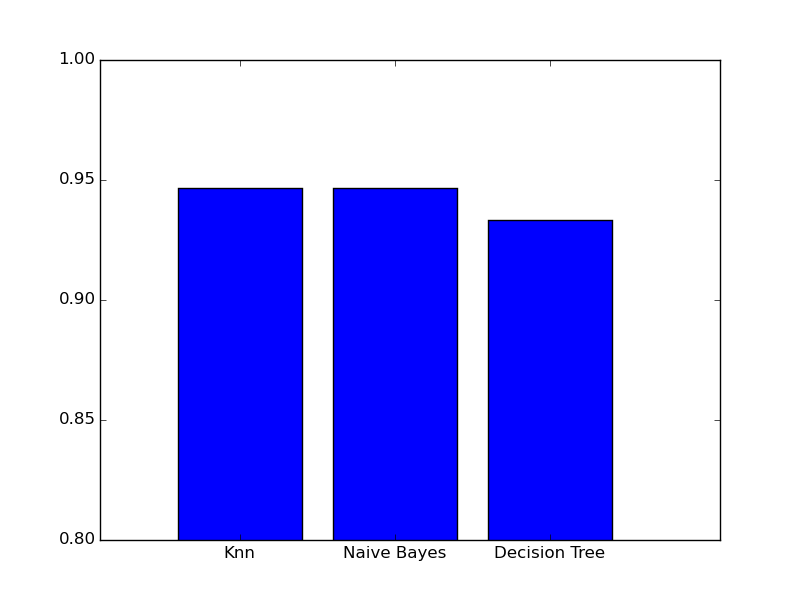
\includegraphics[width=0.5\textwidth]{iris/acuracias.png}
\end{figure}

\begin{figure}[!htb]
  \caption{Escolha do número de vizinhos mais próximos}
  \centering
    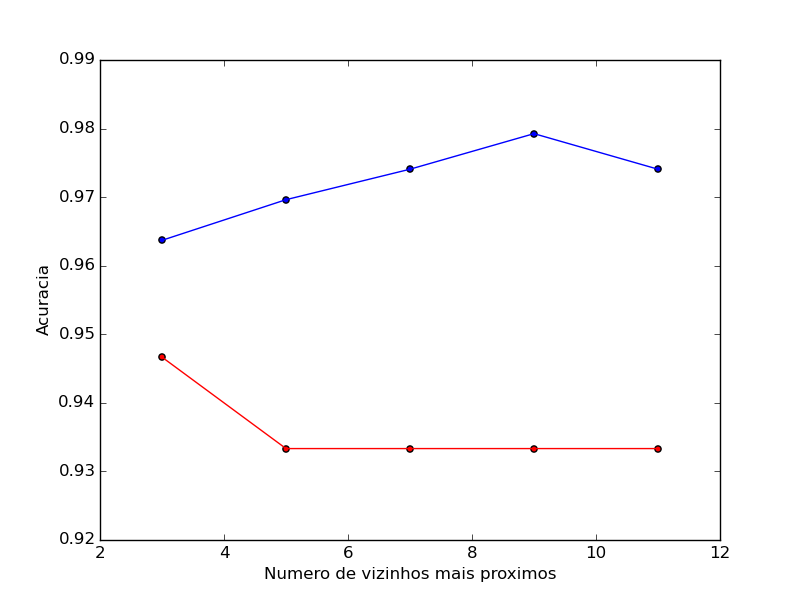
\includegraphics[width=0.5\textwidth]{iris/knn.png}
\end{figure}

\begin{figure}[!htb]
  \caption{Árvore de decisão gerada}
  \centering
    \includegraphics[width=0.5\textwidth]{iris/arvore.eps}
\end{figure}


\newpage
\bibliography{Trabalho_IA.bib}

\end{document}
